To complement the LSD localizer, which returns a line segment in the middle of
the barcode (hereafter called \emph{best line}), we need to find the barcode's boundaries before we can attempt to
read it.

\subsection{Variation}
The variation boundary finder is the original boundary detection method proposed
in \cite{Creusot2016} in conjunction with the LSD localization. Let $L_\perp$
denote the sequence of intensity values along the line perpendicular to the best
line, going through the best line's center (hereafter called \emph{bisector}).
Since barcodes consist of alternating black and white bars, the variation of
intensity values along a line crossing the barcode is expected to be high. The
boundary points are thus expected to have the following property: Extend a 
``probing'' line (\emph{inner probe}) from the boundary point along the bisector, pointing inside the
barcode, i.e. in direction of best line's center. Extend a second ``probing''
line (\emph{outer probe}) from the boundary point in the opposite direction, away from the barcode.
The variation along the inner probe is now expected to be much higher than the
variation along the outer probe.

To find the boundary points, for each index $k$ along the bisector, the signed variation
difference
\begin{equation*}
 \phi_{L_\perp} (k)=\sum_{j=-R}^{0}\abs{L_\perp(k+j)-L_\perp(k+j-1)}-\sum_{j=0}^{R}\abs{L_\perp(k+j)-L_\perp(k+j+1)}
\end{equation*}
is computed. Here, $R$ is the probing distance, which we chose as $R=l_*/2$,
half of the length of the best line.

The right boundary point should lie at the
bisector index with maximal $\phi_{L_\perp}$, while the left boundary point
should have minimal $\phi_{L_\perp}$.

We deviate slightly from \citeauthor{Creusot2016} by instead using the variation
measure
\begin{equation*}
 \phi_{L_\perp}^* (k)=\sum_{j=-R}^{0}\abs{L_\perp(k+j)-L_\perp(k+j-1)}\cdot (R+j)-\sum_{j=0}^{R}\abs{L_\perp(k+j)-L_\perp(k+j+1)}\cdot (R-j)\,,
\end{equation*}
giving higher weight to pixel values near the current boundary candidate at
index $k$.

\subsection{LSD Bound}
Motivated by the high quality of line segments returned by LineSegmentDetector,
we constructed a new boundary finder, using ideas from the variation method
described above. The goal is to determine the line segments corresponding to the two
outer barcode bars, the \emph{boundary segments}.

We first filter the line segments, so that only segments parallel to and located
next to the best
line are kept. To that end, we use the angle criterion and the criterion of sufficient
projected intersection as described in \cref{sec:LSD}. The remaining segments
are sorted based on the position of the projection of their centers onto the
bisector line. The boundary segments should have the following property: As before,
extend an inner probe from the projected center of the boundary segment along the bisector, pointing inside the
barcode. Extend an outer probe in the opposite direction, away from the barcode.
The inner probe is expected to cross a large number of line segments parallel to
and located next to the best line (i.e. segments which have not been
filtered out in the previous step). The outer probe is expected to cross fewer
such lines.
...

\subsection[Wachenfeld]{Wachenfeld \cite{wachenfeld2008robust}}
\begin{figure}[t]
\center
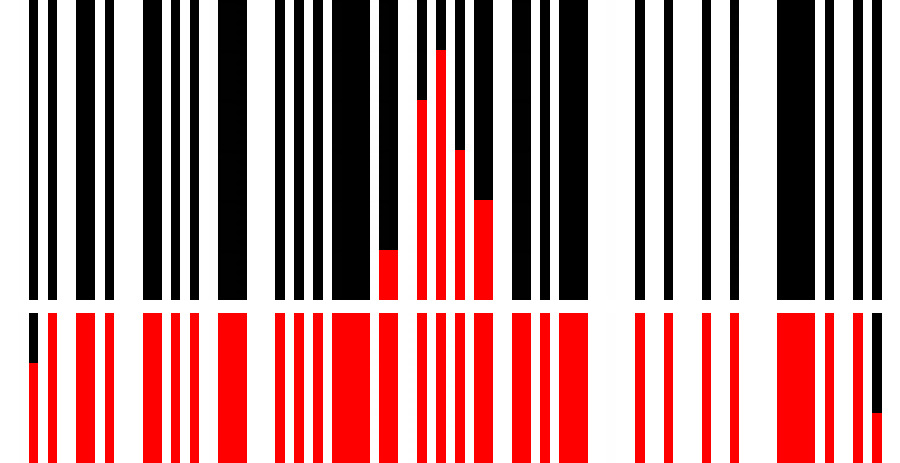
\includegraphics[width=0.6\textwidth,natwidth=900,natheight=463]{img/wachenfeld.png}
\caption{Wachenfeld}
\label{wachenfeld}
\end{figure}
Abbildun \ref{wachenfeld}

%%% Local Variables:
%%% mode: latex
%%% TeX-master: "00Ausarbeitung.tex"
%%% End: